\section{The Thorin phase diagram}\label{cp:sec:phase}

Theorem~\ref{cp:thm:transfer} gives every time $t$ its own threshold basepoint, $\alpha^*(t)=\max(\frac12,\sup\re\rho)$ over the zeros of $\xi_t$, and the set of points at which the shifted clock is a GGC is the region above the graph of $\alpha^*$.

\begin{definition}\label{cp:def:G}
The \emph{GGC region} $\mathcal G$ is the set of points $(t,\alpha)$ with $t\ge0$ and $\alpha\ge\frac12$ at which the shifted clock $\varphi_{t,\alpha}$ is the Laplace transform of a GGC, where at $\alpha=\frac12$ the clock is $R_t$ of Section~\ref{ch:dbn}.
\end{definition}

By Theorem~\ref{cp:thm:transfer}, $(t,\alpha)\in\mathcal G$ exactly when every zero $x+iy$ of $H_t$ has $|y|\le2(\alpha-\frac12)$; at $\alpha=\frac12$ this is the statement that the zeros are real, which is the GGC property of $R_t$ (Theorem~\ref{rz:thm:dbn} for real zeros, Corollary~\ref{bh:cor:dbn} and the pole argument of Theorem~\ref{cp:thm:transfer} for the converse). The slice $t=0$ of $\mathcal G$ concerns the basepoint family of Section~\ref{mw:sec:basepoint}, a GGC for $\alpha\ge\sup\re\rho$ and unconditionally for $\alpha\ge1$, and the slice $\alpha=\frac12$ the flow family $R_t$ of Section~\ref{ch:dbn}, known to be a GGC unconditionally only for $t\ge0.2$ (Problem~\ref{mw:prob:flow}); the diagram joins these two one parameter families. The region is closed upward in $\alpha$, since the threshold condition is monotone. The flow moves it in a definite way.

\begin{theorem}[de Bruijn's strip theorem in Thorin form]\label{cp:thm:phase}
\begin{enumerate}
\item[(i)] If $(t_0,\alpha_0)\in\mathcal G$, then $(t,\alpha)\in\mathcal G$ for every $t\ge t_0$ and every $\alpha\ge\frac12$ with
\[
(\alpha-\tfrac12)^2+\tfrac t2\ \ge\ (\alpha_0-\tfrac12)^2+\tfrac{t_0}2 .
\]
\item[(ii)] $\Lambda=\min\{\,t+2(\alpha-\frac12)^2:(t,\alpha)\in\mathcal G\,\}$.
\item[(iii)] RH holds if and only if $(0,\frac12)\in\mathcal G$, and if and only if $(t,\frac12+\sqrt{\delta-t}/\sqrt2)\in\mathcal G$ for every $\delta>0$ and some $t\in[0,\delta]$.
\end{enumerate}
\end{theorem}

\begin{proof}
De Bruijn's theorem on strips \cite[Theorem 13]{deBruijn}, in the form used by Polymath15 \cite{Polymath}, says that if the zeros of $H_{t_0}$ lie in $|\im z|\le\Delta$, then the zeros of $H_t$ lie in $(\im z)^2\le\max(\Delta^2-2(t-t_0),0)$ for $t\ge t_0$. With $\Delta=2(\alpha_0-\frac12)$ the zeros of $H_t$ then satisfy $|\im z|\le2(\alpha-\frac12)$ whenever $4(\alpha-\frac12)^2\ge4(\alpha_0-\frac12)^2-2(t-t_0)$, which is (i). For (ii), a point $(t,\alpha)\in\mathcal G$ puts the zeros of $H_t$ in $|\im z|\le2(\alpha-\frac12)$, so by (i) those of $H_{t'}$ are real for $t'=t+2(\alpha-\frac12)^2$, and $\Lambda\le t+2(\alpha-\frac12)^2$. Conversely $\Lambda\ge0$ \cite{RodgersTao}, the zeros of $H_\Lambda$ are real, and so $(\Lambda,\frac12)\in\mathcal G$, where the quantity equals $\Lambda$. (iii) The first equivalence is (ii) with $\Lambda\ge0$. For the second, the points named lie on the level set $t+2(\alpha-\frac12)^2=\delta$, so their membership gives $\Lambda\le\delta$ for every $\delta>0$, and conversely RH puts $(0,\frac12)$ in $\mathcal G$, from which (i) gives every point of every level set. For $t=\delta$ the second equivalence is the equivalence of RH with the GGC property of $R_t$ for arbitrarily small $t>0$ in Theorem~\ref{rz:thm:dbn}.
\end{proof}

The quantity $t+2(\alpha-\frac12)^2$ is the natural coordinate on the diagram: it is conserved, in the sense of (i), along the parabolas on which the flow carries the boundary of a certified region, and its minimum over $\mathcal G$ is $\Lambda$. The case $t=0$ of (ii), a zero free half plane $\re s>\alpha$ giving $\Lambda\le2(\alpha-\frac12)^2$, is recorded in Section~\ref{ch:dbn}; the theorem adds the second coordinate, so that certificates at positive time and half planes at time zero are points of one picture and can be compared.

\begin{corollary}[The known region]\label{cp:cor:known}
The following points lie in $\mathcal G$, and with them every point that Theorem~\ref{cp:thm:phase}(i) carries them to; the bounds on $\Lambda$ in (a) to (c) are those of Table~\ref{tab:ch21:hist}.
\begin{enumerate}
\item[(a)] $(0,1)$, by the critical strip; it gives de Bruijn's $\Lambda\le\frac12$.
\item[(b)] $(0.2,0.6)$, by the certificate of Polymath15 \cite{Polymath}; it gives $\Lambda\le0.22$.
\item[(c)] A point on the level set $t+2(\alpha-\frac12)^2=0.2$, by the certificate of Polymath15 with the verification of Platt and Trudgian \cite{PT21}; it gives $\Lambda\le0.2$.
\item[(d)] Conditionally on the half plane announced in October 2026 \cite{OAI26a}, $(0,\frac78)$; it gives $\Lambda\le\frac9{32}$.
\end{enumerate}
\end{corollary}

\begin{proof}
(a) is the absence of zeros of $\zeta$ in $\re s\ge1$ and the functional equation. (b) is the statement proved in \cite{Polymath}: $H_{0.2}$ has no zeros with $\im z>0.2$, which is $(0.2,0.6)\in\mathcal G$. (c) is \cite{PT21}, which takes a row of the table of \cite{Polymath} whose hypothesis their verification satisfies. (d) is immediate from \cite{OAI26a}. The bounds on $\Lambda$ are Theorem~\ref{cp:thm:phase}(ii).
\end{proof}

\begin{figure}[ht]
\centering
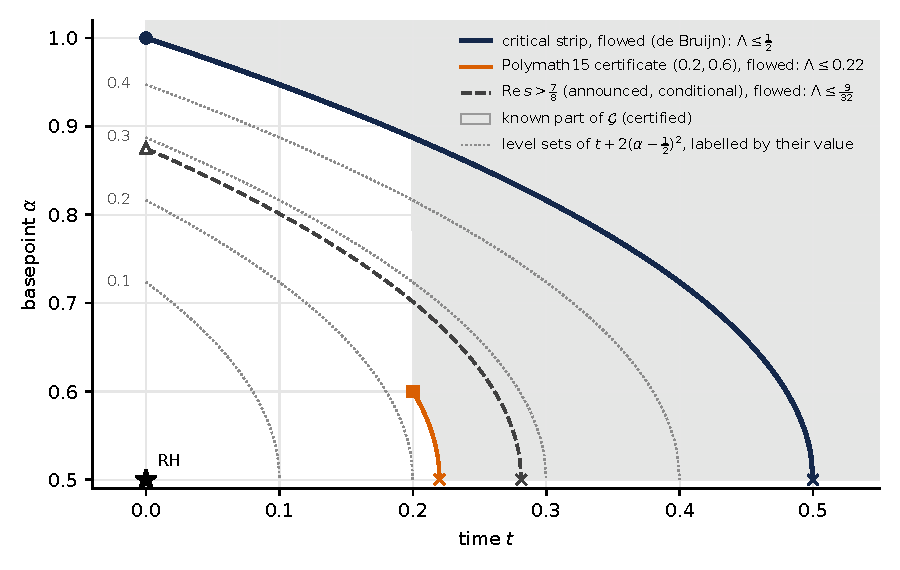
\includegraphics[width=0.85\textwidth]{fig/cp_phase.pdf}
\caption{The Thorin phase diagram. Solid curves are the boundaries of certified GGC regions carried along the flow by Theorem~\ref{cp:thm:phase}(i), and the dashed curve is that of the region conditional on the half plane of Corollary~\ref{cp:cor:known}(d); the dotted curves are the level sets of $t+2(\alpha-\frac12)^2$, labelled by the bound on $\Lambda$ that a point on them gives. RH is the point $(0,\frac12)$. Script \texttt{phase\_thorin.py}.}
\label{cp:fig:phase}
\end{figure}

Figure~\ref{cp:fig:phase} shows the region. The flowed critical strip reaches the axis $\alpha=\frac12$ at $t=\frac12$, the flowed half plane at $t=\frac9{32}$, and the flowed Polymath certificate at $t=0.22$. A half plane at time zero improves the current bound only below $\alpha=\frac12+\sqrt{0.1}\approx0.816$, as Section~\ref{ch:dbn} notes, and on the diagram this is the point where the level set $0.2$ meets the axis $t=0$.

\begin{remark}[Two semigroups]\label{cp:rem:semigroups}
The two coordinates of the diagram carry two monotonicities, and they run in compatible directions. In $\alpha$ the Cauchy densities form a semigroup, so when no zero of $\xi_t$ lies to the right of $\alpha$ the Thorin density at a basepoint $\alpha'>\alpha$ is the Poisson smoothing of the one at $\alpha$, and positivity propagates to the right; going left is deconvolution, which does not preserve positivity (Section~\ref{ag:sec:exactly}). In $t$ the heat flow carries real zeros to real zeros and narrows strips, so membership propagates forward in time. RH asks for the corner where both coordinates are smallest, and neither semigroup can be run backward. The diagram thus places the obstruction of Section~\ref{ag:sec:exactly} and the theorem of Rodgers and Tao in one picture: the region has no slack at the corner, since $\Lambda\ge0$, and if RH is true the corner lies on its boundary.
\end{remark}
